

%%%------------------------------------------------Entwurf -------------------------------------------------------------
\chapter{Entwurf}

\section{Gesamtsystem}
\begin{center}
%\subsubsection*{}%\vspace{3cm}
{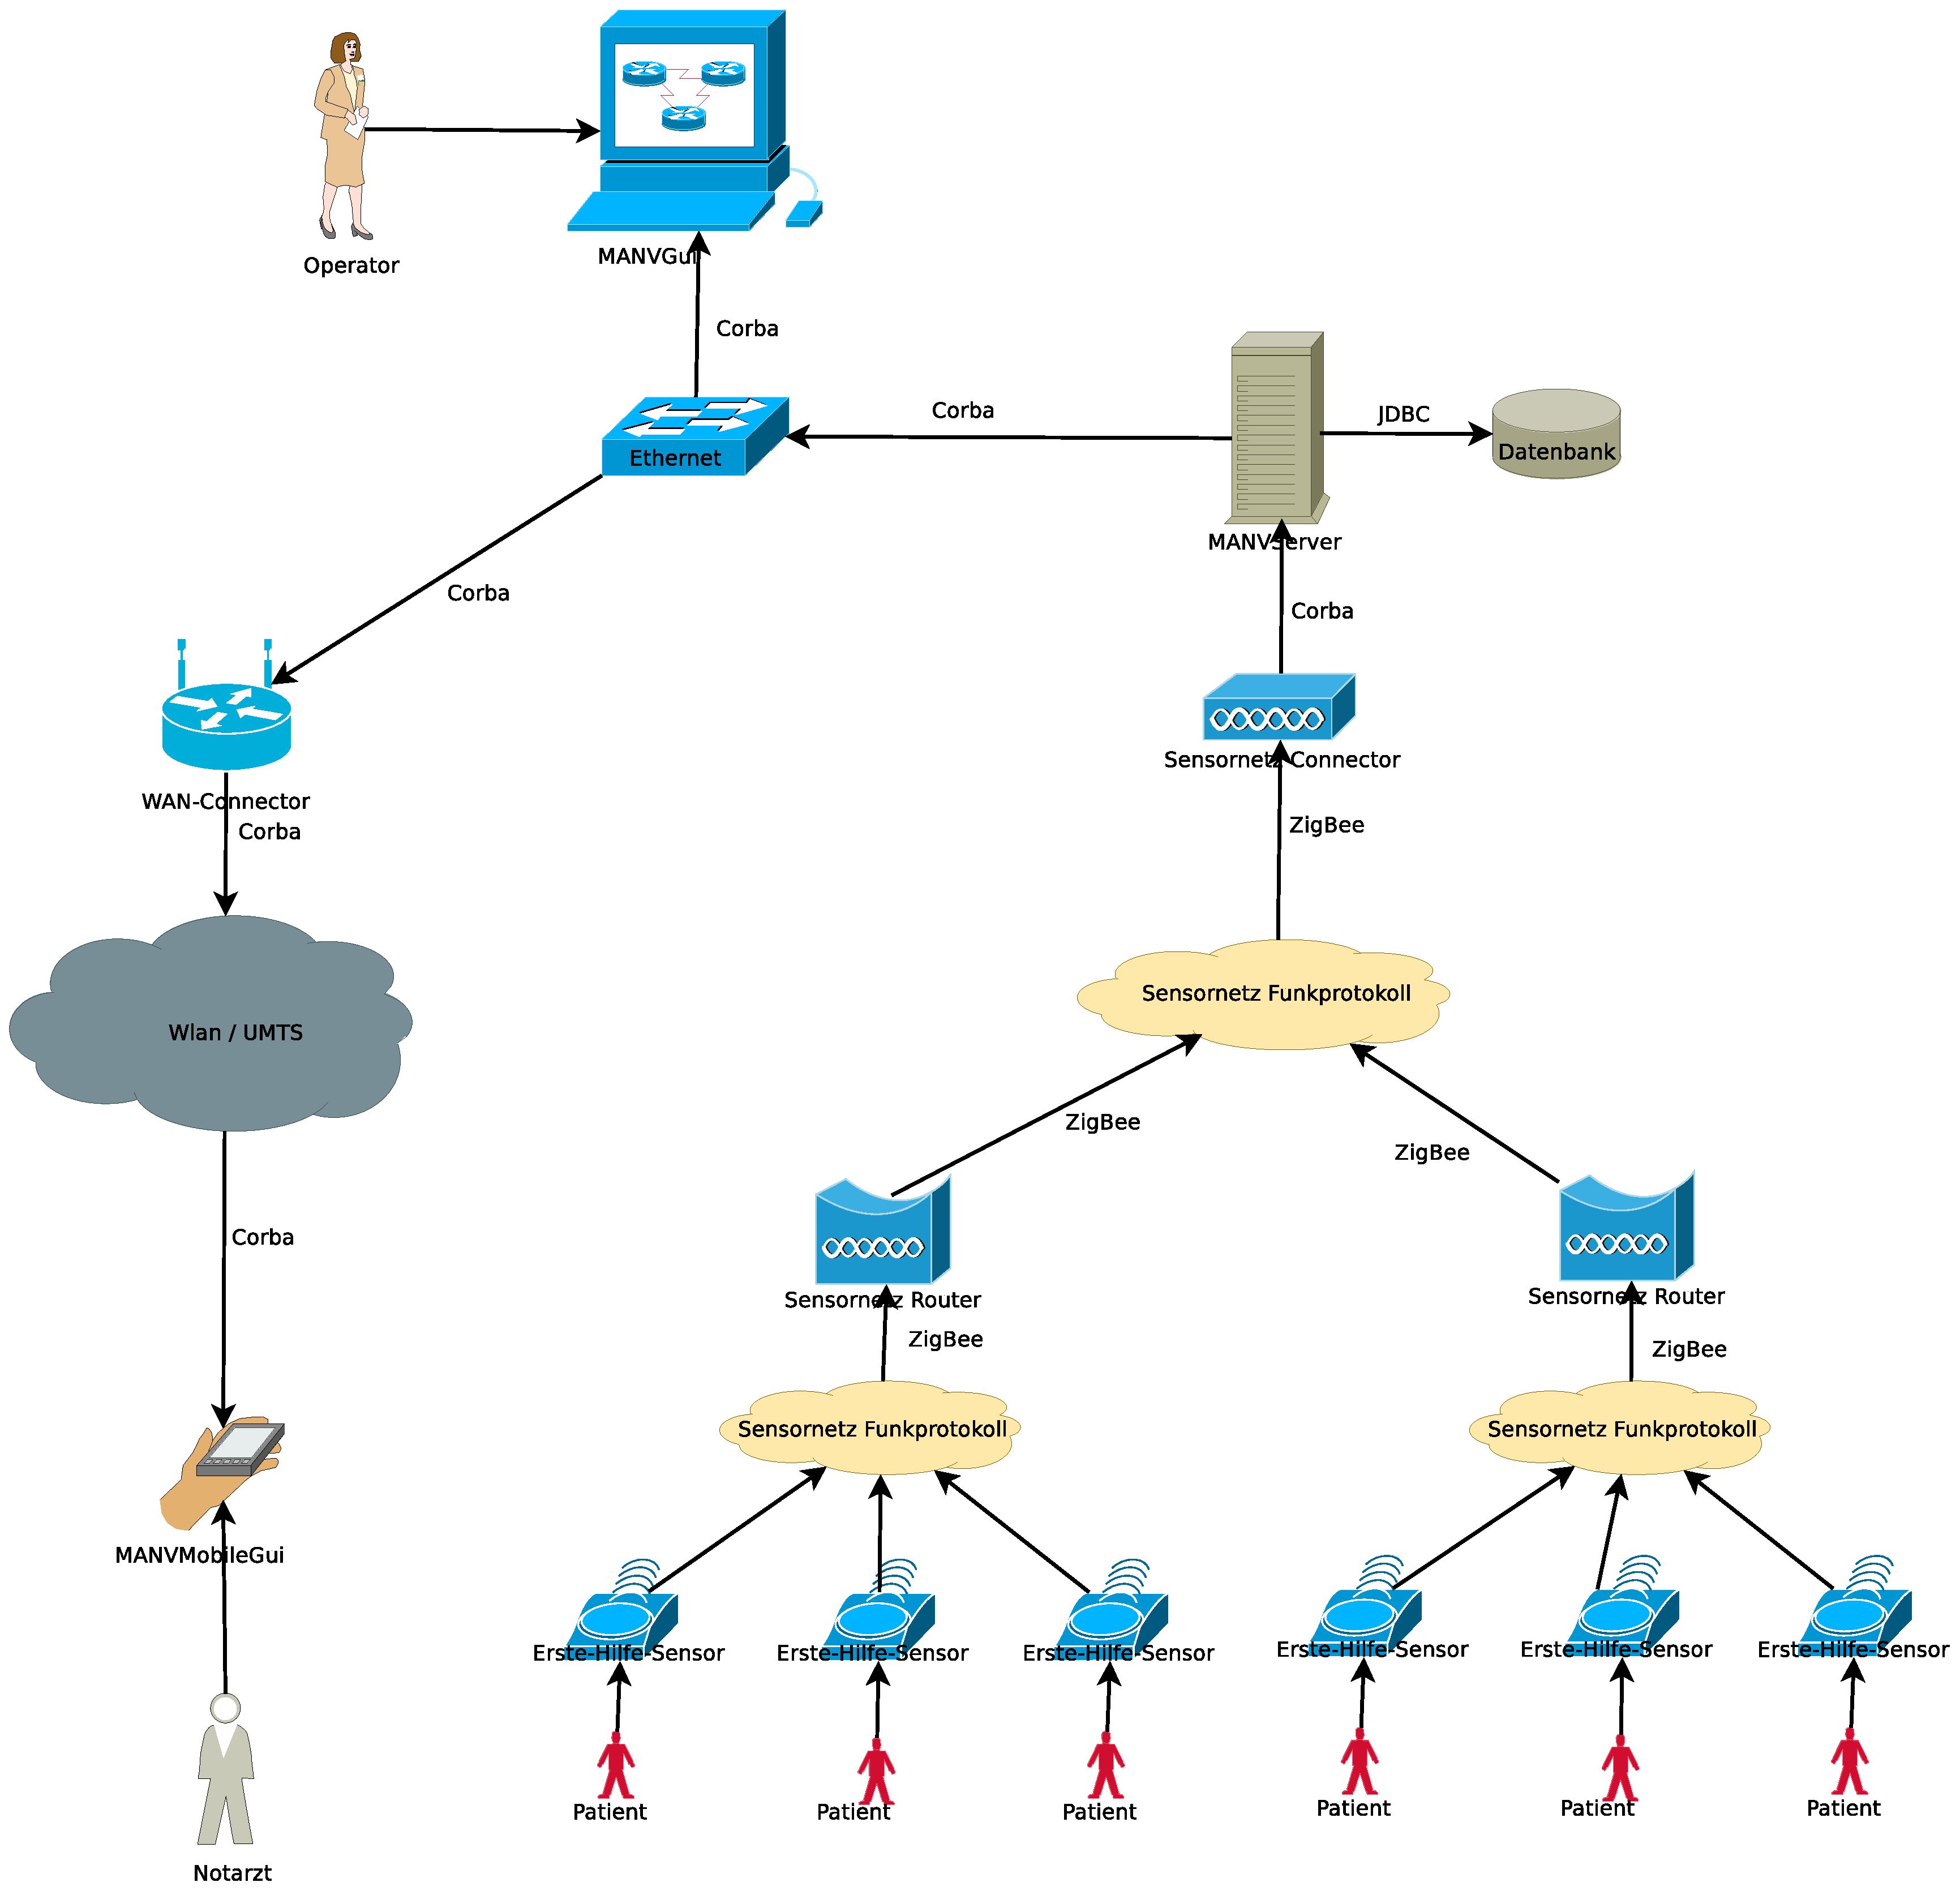
\epsfig{file=diagramme/gesamtuebersicht.eps, scale=0.25}}
\end{center}


\section{Hardware}
\subsection{MANVNode}

\subsection{ADuC}
Beim MANVNode handelt es sich um ein Prototyp des späteren Erste-Hilfe-Sensor für den MANV-Einsatz. Zwar exisitert der 
Erste-Hilfe-Sensor bereits, allerdings hat dieser noch keinerlei Netzwerkfähigkeit. Der Erste-Hilfe-Sensor basiert
auf einem ADuC7019 Microcontroller und ergänzt diesen durch Detektionskomponeten, zur Patientenüberwachung.

Für die Entwicklung der Netzwerkanbindung sind diese Detektionskomponenten nur insofern relevant, dass es zu keiner
Gegenseitigen Störung zwischen Detetion- und Netzwerkkomponeten kommen darf. Daher wurde im ersten Schritt alle nicht
benötigten Komponenten weggelassen, und lediglich der reine Mikrocontroller verwendet. Später wurden die hierbei
entwickelte Netzwerkkomponenten zusammengefasst und in die Hardware des Erste-Hilfe-Sensors integriert.

Die eigentliche Entwicklung fand mit Hilfe eines ADuC7026 Evaluations-Board statt. Dieses Board hat den Vorteil, 
dass alle Anschlüsse des Mikrocontrollers auf Steckerleisten geführt, und damit leicht zugänglich sind. Ausserdem
ist eine JTAG-Schnittstelle vorhanden, die ein einfaches Debuggen des Mikrocontrollers ermöglicht.

\subsection{ZigBee-Schnittstelle}
Für die Anbindung des Erste-Hilfe-Sensors an das Sensornetz wird ein ZigBit-Modul der Firma Atmel verwendet. 
Dieses Modul bietet den Vorteil, dass es bereits über einen kompletten ZigBee-Stack verfügt, der einfach über
AT-Befehle gesteuert werden kann, die per UART gesendet werden.

Der ZigBee-Stack auf dem ZigBit Modul ist austauschbar und kann durch eine eigene Firmware ersetzt werden.
Hierzu wird von der Firma Atmel ein umfangreiches SDK\footnote{Software-Development-Kit: Eine Art Baukasten für
Software, die viele benötigte Teile bereits fertig zur Verfügung stellt} angeboten. Für den Rahmen dieser Diplomarbeit
ist die vorgefertigte Serial-Net-Firmware allerdings ausreichend. Einziger Wermutstropfen ist die fehlende
Verschlüsselung, welche für den Serieneinsatz natürlich erforderlich wäre.

Die Kommunikation mit dem ZigBit Modul erfolgt grundsätzlich synchron. Jeder AT-Befehl wird entweder mit 
"`OK"', "`ERROR"' oder einer Ergebnisszeile quittiert. Der Treiber für das ZigBit-Modul kann also prinzipiell
als endlicher Automat mit zwei Zuständen implementiert werden. Zu beachten ist jedoch, dass prinzipiell
jederzeit Ereignisse vom Typ "`Data Received"' auftreten können. Es ist also notwendig, die Antwort des 
ZigBit Moduls zu parsen, und zu entscheiden, ob es sich um eine Antwort auf einen zuvor gesendeten Befehl
oder aber um ein Data-Ereigniss handelt. Wichtig ist, dass diese Ereignisse nicht verloren gehen dürfen,
da es sich um Befehle handelt, die von der MANVSuite an den Sensor gesendet wurden, und von diesem 
abgearbeitet werden müssen. 


\subsection{Firmware}
Die Firmware des Erste-Hilfe-Sensors wurde um einen Treiber für das ZigBit-Modul ergänzt. Die Firware wurde in der
Programmiersprache C geschrieben, und setzt direkt auf die Hardware des ADuC auf. Es wurde lediglich die von 
Rowley Crossworks angebotene Standardbibliothek verwendet, die einige praktische Funktionen wie Stringmanipulation,
einen Interrupthandler und einen fertigen Startup-Code bietet.

Die Entwicklung von Software für einen Microcontroller zeichnet sich durch die Abwesenheit eines Betriebssystems 
aus. Ein Großteil der Funktionalität, die man von der Entwicklung von Software für einen standard Mikrocomputer 
gewohnt ist, ist schlichtweg nicht vorhanden. Hier sind insbesondere eine automatische Speicherverwaltung sowie
Threads und Prozesse zu erwähnen. Da der Erste-Hilfe-Sensor viele Aufgaben gleichzeitig erfüllen muss, stellt 
dies eine ernst zu nehmende Herausforderung dar. Das Problem wurde durch ein Interrupt getriebenes Programmiermodell
gelöst.

Es werden folgende Interrupts verwendet:

Timer0: Dieser Timer-Interrupt führt die Patientenüberwachung durch. Die einzelnen Sensoren werden abgefragt,
und eine Analyse der empfangenen Daten wird durchgeführt.

Timer1: Dieser Interrupt führt einige periodische Aufgaben durch. Zunächst werden die am Sensor vorhandenen
Taster abgefragt (Alarm Stummschalten, Alarm manuell auslösen etc.). Danach wird überprüft, in welchem Zustand
der Sensor sich aktuell befindet, also z.B. ob ein Alarm aufgetreten ist, oder ob der Patient sich in einem
guten Zustand befindet. Abhängig hiervon werden nun LEDs und ein angeschlossener Piezzo-Summer geschaltet,
um den Zustand nach aussen zu signalisieren. Zu letzt wird noch überprüft, wann zuletzt eine Übertragung
des Zustands des Sensors an die MANVSuite erfolgt ist. Liegt dies länger als einen konfiguriertes Zeitintervall
zurück, so wird eine Übertragung des aktuellen Zustands veranlasst.

Ein weiteres Problem sind die sehr beschränkten Ressourcen des Mikrocontrollers. Insbesondere der Speicher ist
mit 16kB sehr knapp bemessen. 

\subsubsection{UART}
Der ADuC verfügt über einen UART Interrupt, welcher eine Statusänderung des UARTs signalisiert. Im Register 
\textsl{COMIEN0} wird konfiguriert, welche Zustände über den Interrupt singnalisiert werden sollen. Tritt
nun einer dieser Zustände auf, so wird der UART Interrupt ausgelöst. Im Interrupthandler muss nun überprüft
werden, welches Ereigniss zum Auslösen des Interrupts geführt hat. Dies ist im Register \textsl{COMSTA0} 
gespeichert. Wichtig ist an dieser Stelle, dass auch mehrere Ereignisse gleichzeitig auftreten können. 
Dies muss im Interrupthandler berücksichtigt werden, da sonst Ereignisse verloren gehen können.

Das eigentliche Senden und Empfangen erfolgt über die beiden Register \textsl{COMRX} und \textsl{COMTX}.
Zum Senden wird hierzu ein einzelnes Zeichen in \textsl{COMTX} gelegt. Nun muss eine gewisse Zeit gewartet
werden, bis das Zeichen gesendet wurde, und das nächste Zeichen in \textsl{COMTX} gelegt werden kann.
FÜr das Empfangen wird das Register \textsl{COMRX} in analoger Weise verwendet werden. Ob das nächste
Zeichen empfangen bzw. gesendet werden kann, kann mit Hilfe der Bits \textsl{DR} ("`Data Ready"' - Daten liegen vor)
bzw. \textsl{TEMT} ("`Transmit Buffer empty"' - Daten können gesendet werden) bestimmt werden.

Die einfachste Methode wäre hierbei, in einer Schleife Busy-Waiting zu betreiben, und so lange zu warten,
bis sich eins der beiden Bits verändert. Dies wäre jedoch sehr aufwendig und würde den Mikrocontroller 
unnötig lange blockieren. Statt dessen wird der Zustand der beiden Register nur dann überprüft, wenn ein 
UART-Interrupt aufgetreten ist.

Zum Senden und Empfangen von Daten werden zwei Ringpuffer verwendet. Möchte ein Unterprogramm Daten senden,
so greift es nicht direkt auf die UART-Schnittstelle zu sondern legt diese Daten lediglich in den Sendepuffer.
Das eigentliche Senden wird nun vom UART-Interrupthandler durchgeführt; das Unterprogramm kann weiter arbeiten,
ohne auf das fertige Senden der Daten warten zu müssen.

Das Empfangen von Daten erfolgt analog. Jedesmal wenn ein Zeichen von der seriellen Schnitstelle empfangen
wurde, wird dieses in den Empfangspuffer gelegt. Das Abarbeiten des Empfangspuffer erfolgt nun als Idle-Task:
Immer dann, wenn der Mikrocontroller gerade keine anderen Aufgaben erfüllen muss, wird der Empfangspuffer
abgearbeitet und eventuell empfangene Befehle werden abgearbeitet. Dies kann natürlich jederzeit durch 
die Abarbeitung von Interrupts unterbrochen werden.

\subsubsection{MANV-USB-Connector}
Der MANV-USB-Connector ist die Schnittstelle zwischen Sensornetz und Computer. Es handelt sich um einen USB-Stick, der einen
ZigBit-Modul beinhaltet. Zusätzlich sind zwei weitere Bauteile enthalten, die das ZigBit-Modul mit Strom versorgen, sowie eine
Umsetzung der UART-Schnittstelle des ZigBit-Moduls auf USB vornehmen. Für die Stromversorgung ist es notwendig, die 5V der
USB-Schnittstelle auf die 3V des ZigBit-Moduls umzusetzen.

\subsection{Software}

In dieser Arbeit wurde ein Java-Treiber (MANVConnector) entworfen und implemtiert. Dieser Treiber realisiert die die Anbindung an
die von Herrn Tepelmann in \cite{Jan} entwickelte MANVSuite.

Der MANVConnector hat einerseits die Aufgabe, Daten die von dem MANV-USB-Connector empfangen wurden in Corba-Events 
umzusetzen, und an den MANVServer weiterzuleiten. Andererseits empfängt sie Corba-Events vom MANVServer, dekodiert
diese und sendet diese in Form von Sensornetz Befehlen an die zuständigen MANVNodes weiter.

Bei der Kommunikation mit dem auf dem USB-Stick aufgebrachten ZigBee-Modul stellen sich grundsätzlich die selben 
Synchronisierungsprobleme wie in der MANVFirmware. Da der MANVConnector jedoch alle Möglichkeiten der Java-Virtual-Machine
nutzen kann, lassen sich diese deutlich einfacher und eleganter lösen.

Analog zu den Sende- und Empfangspuffern in der Firmware gibt es im MANVConnector drei Queues:

\begin{itemize}
    \item{Die Command Queue:} In dieser Queue werden alle zu sendenden Befehle gespeichert.
    \item{Die Event Queue:} In dieser Queue werden alle empfangenen Ereignisse gespeichert.
    \item{Die Result Queue:} In dieser Queue werden alle bereits gesendeten Befehle zusammen mit dem
                             Resultat, das dieser Befehl hatte, gespeichert.
\end{itemize}

Jedes Element der einzelnen Queues verfügt über eine Priorität; die Queues sorgen dafür, dass der
Zugriff nach Priotität sortiert erfolgt. Hierdurch wird sicher gestellt, dass wichtige Ereignisse
wie z.B. ein Alarm bevorzugt ausgeliefert werden.

Der MANVConnector ist in drei Threads aufgeteilt:

\begin{itemize}
    \item{SocketWriter:} Dieser Thread entnimmt Befehle aus der \textsl{CommandQueue} und sendet
                         diese über den MANV-USB-Connector an das Sensornetz. Nun blockiert der
                         Thread so lange, bis das Ergebnis des Befehls zur Verfügung steht.
                         Sobald dies der Fall ist, wird der Befehl zusammen mit dem Ergebnis in
                         die \textsl{ResultQueue} eingefügt.
    \item{SocketReader:} Dieser Thread empfängt Daten aus dem Sensornetz. Handelt es sich um ein
                         Ergebnis, so wird dies dem \textsl{SocketWrite} signalisiert, und das
                         Ergebnis zur Abholung durch den \textsl{SocketWriter} zur Verfügung
                         gestellt. Handelt es sich hingegen um einen Ereignis, so wird dieses
                         in die \textsl{EventQueue} eingefügt.
    \item{Haupt-Thread:} Dieser Thread ist für die Kommunikation mit MANVServer zuständig.
                         Befehle, die vom MANVServer empfangen werden, werden für das 
                         Sensornetz aufbereitet und in die CommandQueue eingestellt.
                         Ausserdem werden Ereignisse aus der \textsl{EventQueue} entnommen,
                         in Corba-Events übersetzt und an den MANVServer zugestellt.
\end{itemize}                          

\subsection{Automatisches Failover für den ZigBee Coordinator}

\section{Implementierung}

\subsection{Hardware}

\subsection{Firmware}

\subsection{Software}


